Et verktøy for å visualisere hvordan gruppens medlemmer står i forhold til hverandre kaller samarbeidsindikatorer. 
Verktøyet er utarbeidet av Are Holden i samarbeid med EiT-satben. 
Dette var et tilbud alle gruppene i landsbyen fikk og testen ble gjennomført av fasilitatorene. 
Undersøkelsen ble gjennomført ved at vi svarte på en rekke spørsmål anonymt. 
Disse svarene ble da grunnlaget for en graf som kalles samarbeidsindikatorer. 
Denne grafen belyser områder som gruppen har små, middels eller store utfordringer. 
For å oppdage eventuell fremgang ble denne testen gjort to ganger iløpet av EiT, en gang helt i begynnelsen (2. landsbydag) og en gang mot slutten av prosjektet (10. landsbydag). 

\subsection{2. landsbydag}
På grunn av at den første testen ble tatt i en tidlig fase av gruppearbeidet, gir den et godt intrykk av gruppens initielle situasjon. 
På grafen er det to linjer, en heltrukken rød og en en striplet rød. 
Disse linjene markerer grensene på hvor ting blir regnet som store problemer og små problemer. 
\begin{figure}[H]
    \centering
    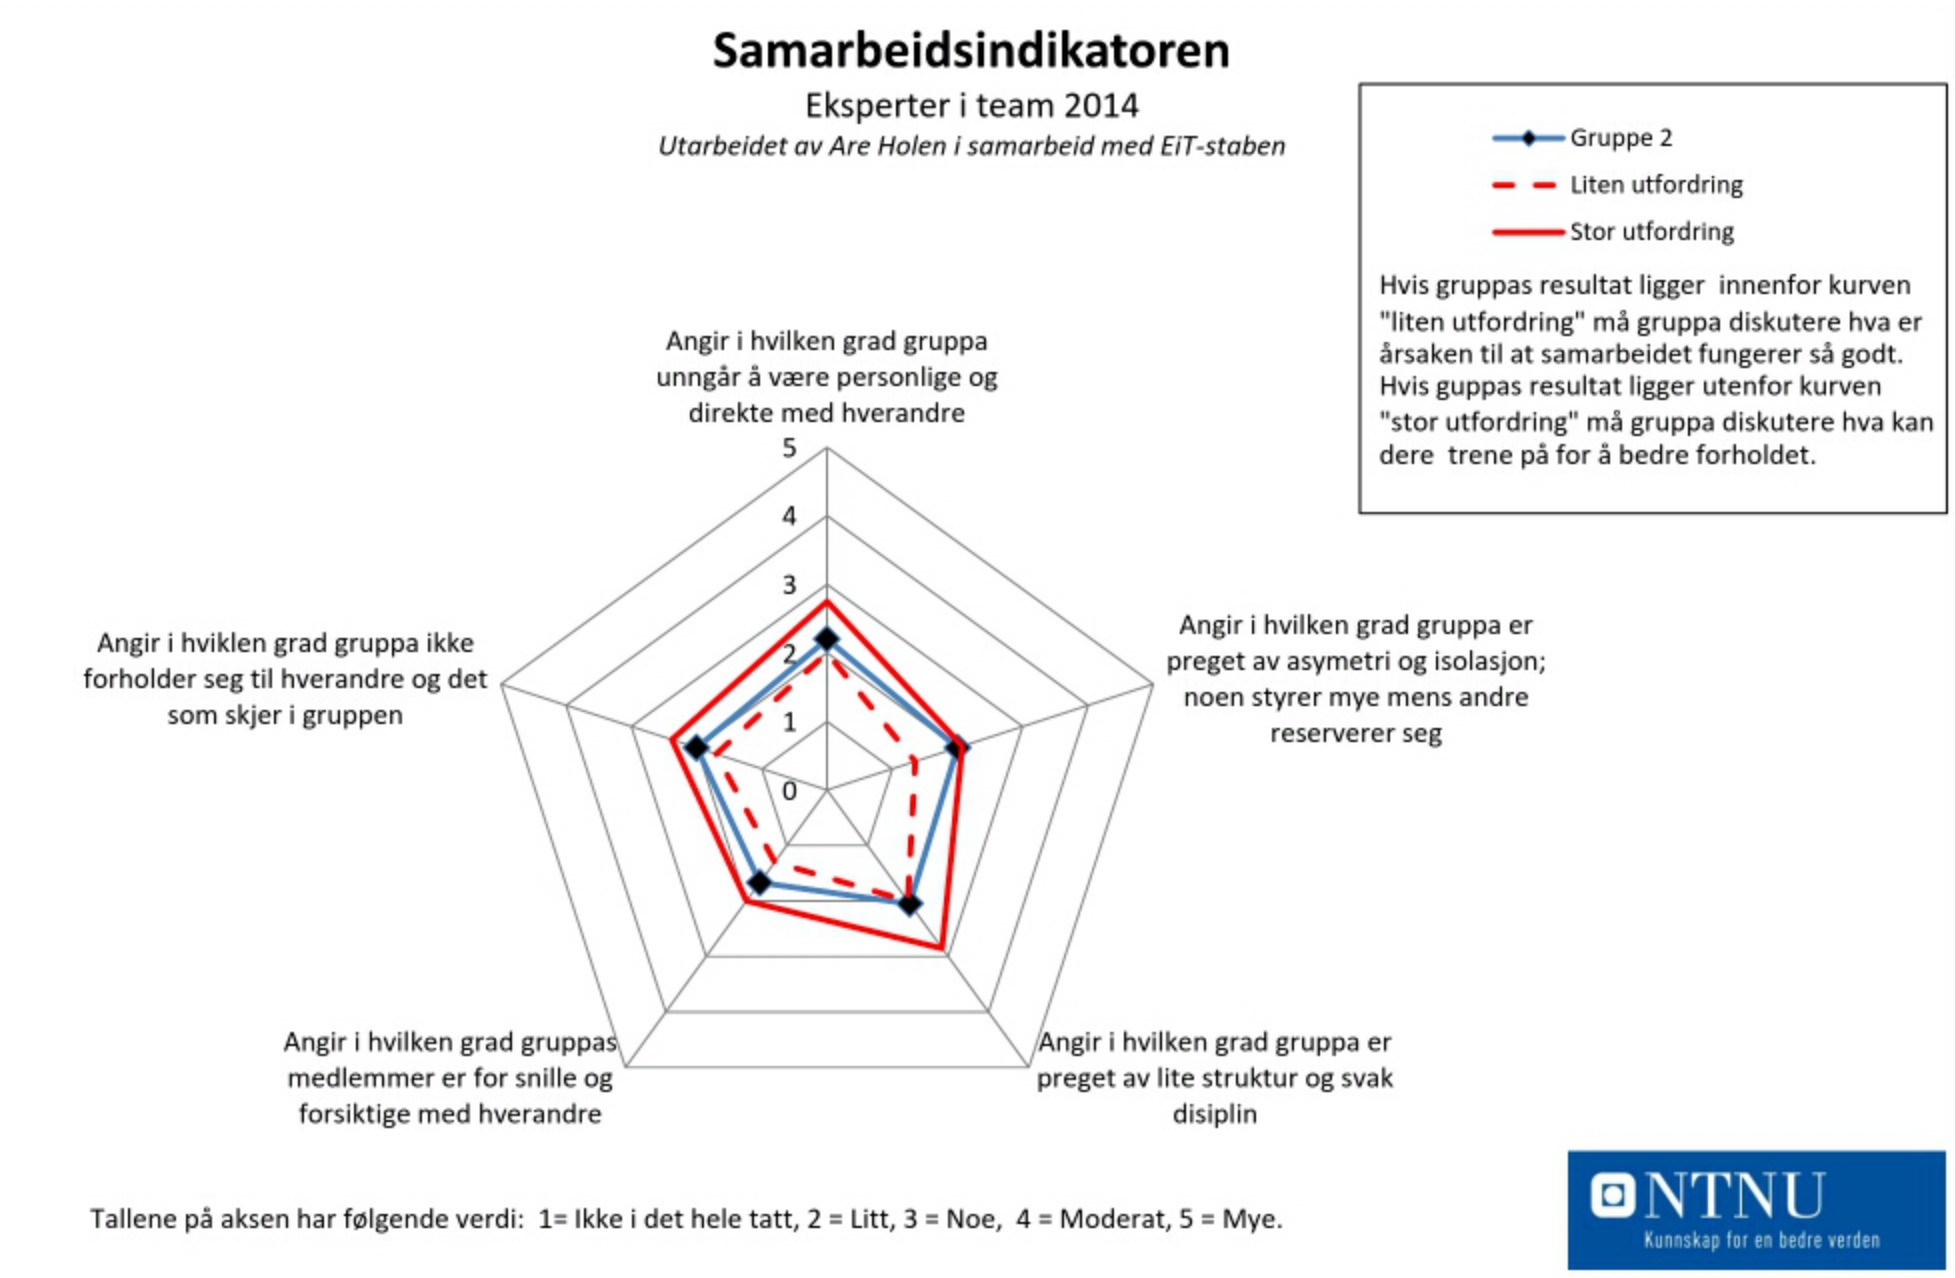
\includegraphics[width=0.7\textwidth]{images/samarbeidsindikator1.jpeg} 
    \caption{Samarbeidsindikatorer 2. landsbydag}
    \label{fig:sam1}
\end{figure}

\noindent \textbf{Hvilken grad gruppen unngår å være personlig:} 2.2.
\newline
\noindent Blablabla
\vspace{\secspace}

\noindent \textbf{hvilken grad gruppen er preget av asymetri ogisolasjon:} 2.
\newline
\noindent Blablabla
\vspace{\secspace}

\noindent \textbf{Hvilken grad gruppen er preget av lite struktur:} 1.
\newline
\noindent Blablabla
\vspace{\secspace}

\noindent \textbf{Hvilken grad gruppen er for snille med hverandre:} 1.8.
\newline
\noindent Blablabla
\vspace{\secspace}

\noindent \textbf{Hvilken grad gruppen ikke forholder seg til hverandre:} 1.
\newline
\noindent Blablabla

\subsection{10. landsbydag}
\begin{figure}[H]
    \centering
    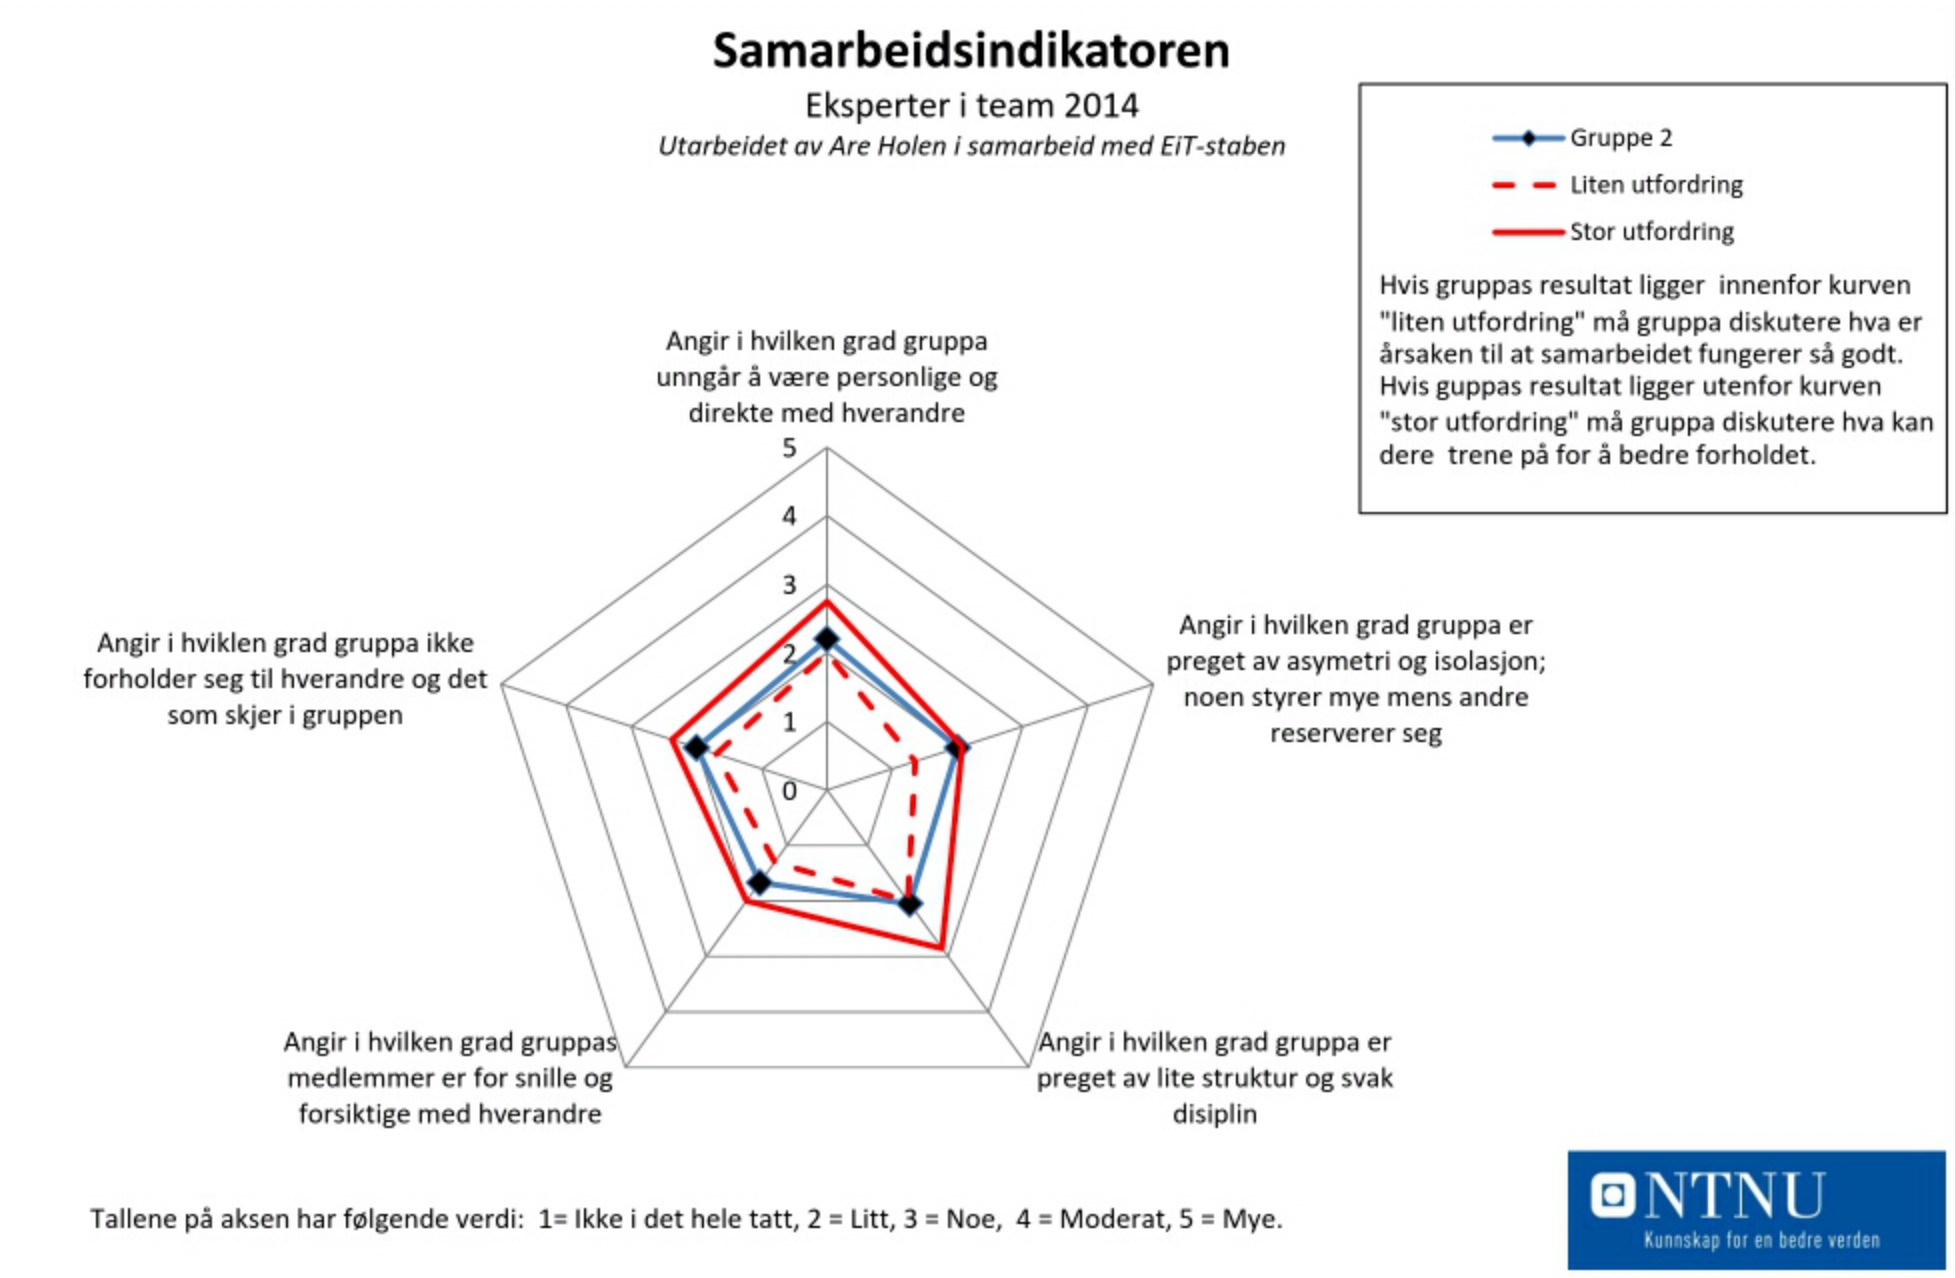
\includegraphics[width=0.7\textwidth]{images/samarbeidsindikator1.jpeg} 
    \caption{Samarbeidsindikatorer 10. landsbydag}
    \label{fig:sam2}
\end{figure}